% =========================================================================
% BÀI 28: LUYỆN TẬP CHUNG (CHỦ ĐỀ 7 - ĐỘ DÀI VÀ ĐO ĐỘ DÀI - TOÁN LỚP 1)
% TOÀN BỘ CÂU HỎI ĐƯỢC VẼ HÌNH MINH HỌA TRỰC QUAN 100% BẰNG TIKZ 2D & 3D
% =========================================================================

% --- CÁC HÀM VẼ HÌNH TRỰC QUAN ĐẶC TRƯNG CHO BÀI 28 ---

% 1. Thước kẻ chia cm
\providecommand{\VeThuocCmMini}[3][cyan]{% #1=màu thước, #2=max cm, #3=(x,y)
  \begin{scope}[shift={(#3)}, scale=0.65]
    \draw[fill=#1!20, draw=black!80, line width=0.7pt, rounded corners=2pt] (-0.3,-0.5) rectangle (#2+0.4,0.5);
    \node[font=\bfseries\tiny, color=#1!80!black] at (-0.05,-0.25) {cm};
    \foreach \x in {0,1,...,#2} {
      \draw[black!85, line width=0.5pt] (\x,0.5) -- (\x,0.18);
      \node[below, font=\tiny\bfseries] at (\x,0.18) {\x};
    }
  \end{scope}
}

% 2. Thanh đo độ dài có màu và số đo
\providecommand{\VeThanhDoDai}[5]{% #1=chiều dài cm, #2=màu, #3=(x,y), #4=nhãn trên, #5=nhãn dưới
  \begin{scope}[shift={(#3)}, scale=0.6]
    \draw[fill=#2!40, draw=black!80, line width=0.6pt, rounded corners=2pt] (0,0) rectangle (#1,0.6);
    \node[font=\bfseries\tiny, color=black] at (#1/2,0.3) {#4};
    \draw[line width=0.7pt, stealth-stealth, black!70] (0,-0.25) -- (#1,-0.25) node[midway, below, font=\bfseries\tiny] {#5};
  \end{scope}
}

% =========================================================================
% BẮT ĐẦU NỘI DUNG 20 CÂU HỎI
% =========================================================================

\textbf{Phần 1. Trắc nghiệm lựa chọn}
\setcounterpageref{ex}{0}

% --- TRANG 1: CÂU 1 ĐẾN CÂU 4 ---

% CÂU 1: Kí hiệu cm
\begin{ex} %[1H7N28]
Quan sát chữ viết tắt trên đầu chiếc thước kẻ học sinh:
\begin{center}\vspace{-2.5mm}
\begin{tikzpicture}
  \VeThuocCmMini[cyan]{6}{0,0}
  \draw[line width=1pt, red!85, ->] (-0.05,0.8) -- (-0.05,0.4) node[above=8pt, font=\bfseries\tiny, color=red!85] {Kí hiệu xăng-ti-mét};
\end{tikzpicture}
\vspace{-2.5mm}\end{center}
Kí hiệu của đơn vị đo độ dài xăng-ti-mét là:
\begin{multicols}{4}
\choice
{$\text{kg}$}
{$\text{m}$}
{\True $\text{cm}$}
{$\text{l}$}
\end{multicols}
\loigiai{
Xăng-ti-mét có kí hiệu viết tắt là $\text{cm}$.\\
\textbf{Đáp án: C.}
}
\end{ex}

% CÂU 2: Phép tính cộng 8 cm + 6 cm
\begin{ex} %[1H7N28]
Hai đoạn que tính được nối tiếp nhau:
\begin{center}\vspace{-2.5mm}
\begin{tikzpicture}[scale=0.6]
  \draw[fill=blue!30, draw=black] (0,0) rectangle (3.2,0.5) node[midway, font=\tiny\bfseries] {$8\text{ cm}$};
  \draw[fill=orange!40, draw=black] (3.2,0) rectangle (5.6,0.5) node[midway, font=\tiny\bfseries] {$6\text{ cm}$};
  \draw[line width=0.8pt, stealth-stealth, red!85] (0,-0.3) -- (5.6,-0.3) node[midway, below, font=\bfseries\tiny] {Tổng cộng = ? cm};
\end{tikzpicture}
\vspace{-2.5mm}\end{center}
Tính: $8\text{ cm} + 6\text{ cm} = \dots$
\begin{multicols}{4}
\choice
{$13\text{ cm}$}
{\True $14\text{ cm}$}
{$15\text{ cm}$}
{$16\text{ cm}$}
\end{multicols}
\loigiai{
$8 + 6 = 14\text{ cm}$.\\
\textbf{Đáp án: B.}
}
\end{ex}

% CÂU 3: Phép tính trừ 17 cm - 7 cm
\begin{ex} %[1H7H28]
Sợi dây dài $17\text{ cm}$, cắt bớt đi một đoạn $7\text{ cm}$:
\begin{center}\vspace{-2.5mm}
\begin{tikzpicture}[scale=0.6]
  \draw[fill=green!40, draw=black] (0,0) rectangle (3.6,0.5) node[midway, font=\tiny\bfseries] {Còn lại ? cm};
  \draw[fill=gray!30, draw=black, dashed] (3.6,0) rectangle (6.0,0.5) node[midway, font=\tiny\bfseries] {Cắt $7\text{ cm}$};
  \draw[line width=0.8pt, stealth-stealth, blue!85] (0,-0.3) -- (6.0,-0.3) node[midway, below, font=\bfseries\tiny] {Ban đầu $17\text{ cm}$};
\end{tikzpicture}
\vspace{-2.5mm}\end{center}
Tính: $17\text{ cm} - 7\text{ cm} = \dots$
\begin{multicols}{4}
\choice
{$9\text{ cm}$}
{$11\text{ cm}$}
{\True $10\text{ cm}$}
{$12\text{ cm}$}
\end{multicols}
\loigiai{
$17 - 7 = 10\text{ cm}$.\\
\textbf{Đáp án: C.}
}
\end{ex}

% CÂU 4: Cộng hai số tròn chục 30 cm + 20 cm
\begin{ex} %[1H7H28]
Ghép hai thanh gỗ tròn chục:
\begin{center}\vspace{-2.5mm}
\begin{tikzpicture}[scale=0.6]
  \draw[fill=yellow!40, draw=black] (0,0) rectangle (3.0,0.5) node[midway, font=\tiny\bfseries] {$30\text{ cm}$};
  \draw[fill=cyan!35, draw=black] (3.0,0) rectangle (5.0,0.5) node[midway, font=\tiny\bfseries] {$20\text{ cm}$};
  \draw[line width=0.8pt, stealth-stealth, red!85] (0,-0.3) -- (5.0,-0.3) node[midway, below, font=\bfseries\tiny] {Cả hai thanh = ? cm};
\end{tikzpicture}
\vspace{-2.5mm}\end{center}
Tính: $30\text{ cm} + 20\text{ cm} = \dots$
\begin{multicols}{4}
\choice
{$40\text{ cm}$}
{\True $50\text{ cm}$}
{$60\text{ cm}$}
{$70\text{ cm}$}
\end{multicols}
\loigiai{
$30 + 20 = 50\text{ cm}$.\\
\textbf{Đáp án: B.}
}
\end{ex}

\newpage
% --- TRANG 2: CÂU 5 ĐẾN CÂU 8 ---

% CÂU 5: Trừ số tròn chục 70 cm - 30 cm
\begin{ex} %[1H7H28]
Cây tre dài $70\text{ cm}$, cưa bớt đi $30\text{ cm}$:
\begin{center}
\begin{tikzpicture}[scale=0.65]
  \draw[fill=teal!30, draw=black] (0,0) rectangle (3.6,0.6) node[midway, font=\bfseries\scriptsize] {Còn lại ? cm};
  \draw[fill=gray!30, draw=black, dashed] (3.6,0) rectangle (6.0,0.6) node[midway, font=\bfseries\scriptsize] {Bớt $30\text{ cm}$};
  \draw[line width=1pt, stealth-stealth, blue!85] (0,-0.35) -- (6.0,-0.35) node[midway, below, font=\bfseries\scriptsize] {Ban đầu $70\text{ cm}$};
\end{tikzpicture}
\end{center}
Tính: $70\text{ cm} - 30\text{ cm} = \dots$
\begin{multicols}{4}
\choice
{\True $40\text{ cm}$}
{$30\text{ cm}$}
{$50\text{ cm}$}
{$60\text{ cm}$}
\end{multicols}
\loigiai{
$70 - 30 = 40\text{ cm}$.\\
\textbf{Đáp án: A.}
}
\end{ex}

% CÂU 6: So sánh biểu thức với số đo
\begin{ex} %[1H7H28]
So sánh hai tấm bảng số đo độ dài:
\begin{center}

\begin{tikzpicture}[scale=0.65]
  \node[draw=blue!80, fill=cyan!15, rounded corners=3pt, font=\bfseries\normalsize, inner sep=4pt] at (-2.2,0) {$15\text{ cm} + 4\text{ cm}$};
  \node[draw=orange!90, fill=yellow!30, rounded corners=2pt, font=\bfseries\normalsize, inner sep=3pt] at (0.2,0) {~?~};
  \node[draw=red!80, fill=pink!20, rounded corners=3pt, font=\bfseries\normalsize, inner sep=4pt] at (2.2,0) {$20\text{ cm}$};
\end{tikzpicture}
\end{center}
Dấu thích hợp để điền vào ô trống so sánh $15\text{ cm} + 4\text{ cm} \dots 20\text{ cm}$ là:
\begin{multicols}{4}
\choice
{$>$}
{$=$}
{\True $<$}
{$+$}
\end{multicols}
\loigiai{
Ta có $15\text{ cm} + 4\text{ cm} = 19\text{ cm}$. Vì $19\text{ cm} < 20\text{ cm}$ nên điền dấu $<$.\\
\textbf{Đáp án: C.}
}
\end{ex}

% CÂU 7: Hai đoạn thẳng nối tiếp
\begin{ex} %[1H7V28]
Đoạn thẳng thứ nhất dài $14\text{ cm}$, đoạn thứ hai dài $5\text{ cm}$:
\begin{center}
\begin{tikzpicture}[scale=0.65]
  \draw[line width=2.5pt, blue!80] (0,0) -- (4.2,0) node[midway, above, font=\bfseries\tiny] {$14\text{ cm}$};
  \draw[line width=2.5pt, orange!90] (4.2,0) -- (5.7,0) node[midway, above, font=\bfseries\tiny] {$5\text{ cm}$};
  \fill[red] (0,0) circle (0.1cm);
  \fill[red] (4.2,0) circle (0.1cm);
  \fill[red] (5.7,0) circle (0.1cm);
  \draw[line width=0.8pt, stealth-stealth, black!70] (0,-0.35) -- (5.7,-0.35) node[midway, below, font=\bfseries\tiny] {Tổng độ dài cả hai đoạn = ? cm};
\end{tikzpicture}
\end{center}
Cả hai đoạn thẳng dài tất cả là:
\begin{multicols}{4}
\choice
{$18\text{ cm}$}
{$20\text{ cm}$}
{$21\text{ cm}$}
{\True $19\text{ cm}$}
\end{multicols}
\loigiai{
Cả hai đoạn dài tất cả là: $14 + 5 = 19\text{ cm}$.\\
\textbf{Đáp án: D.}
}
\end{ex}

% CÂU 8: Cây mía bị chặt bớt
\begin{ex} %[1H7V28]
Cây mía dài $80\text{ cm}$, bố chặt bớt đi $30\text{ cm}$:
\begin{center}
\begin{tikzpicture}[scale=0.65]
  \draw[fill=green!50!teal, draw=black] (0,0) rectangle (4.0,0.6) node[midway, font=\bfseries\scriptsize] {Còn lại ? cm};
  \draw[fill=gray!30, draw=black, dashed] (4.0,0) rectangle (6.4,0.6) node[midway, font=\bfseries\scriptsize] {Bớt $30\text{ cm}$};
  \draw[line width=1pt, stealth-stealth, orange!90!black] (0,-0.35) -- (6.4,-0.35) node[midway, below, font=\bfseries\scriptsize] {Cây mía dài $80\text{ cm}$};
\end{tikzpicture}
\end{center}
Cây mía còn lại dài là:
\begin{multicols}{4}
\choice
{$40\text{ cm}$}
{\True $50\text{ cm}$}
{$60\text{ cm}$}
{$70\text{ cm}$}
\end{multicols}
\loigiai{
Cây mía còn lại dài: $80 - 30 = 50\text{ cm}$.\\
\textbf{Đáp án: B.}
}
\end{ex}

\newpage
% --- TRANG 3: CÂU 9 ĐẾN CÂU 12 ---

% CÂU 9: Biểu thức tính cộng trừ kết hợp
\begin{ex} %[1H7V28]
Dãy tính độ dài trên băng giấy:
\begin{center}

\begin{tikzpicture}[scale=0.7]
  \node[draw=blue!80, fill=cyan!10, rounded corners=3pt, font=\bfseries\normalsize, inner sep=4pt] at (0,0) {
    $12\text{ cm} + 6\text{ cm} - 8\text{ cm} = \dots$
  };
\end{tikzpicture}
\end{center}
Giá trị của biểu thức trên là:
\begin{multicols}{4}
\choice
{\True $10\text{ cm}$}
{$9\text{ cm}$}
{$11\text{ cm}$}
{$12\text{ cm}$}
\end{multicols}
\loigiai{
$12 + 6 = 18\text{ cm}$; sau đó $18 - 8 = 10\text{ cm}$.\\
\textbf{Đáp án: A.}
}
\end{ex}

% CÂU 10: Đo bàn học bằng 6 gang tay
\begin{ex} %[1H7V28]
Đo chiều dài chiếc bàn bằng $6$ gang tay (mỗi gang tay dài $10\text{ cm}$):
\begin{center}
\begin{tikzpicture}[scale=0.6]
  \foreach \k in {0,1,2,3,4,5} {
    \draw[fill=yellow!40, draw=black] (\k*1.1,0) rectangle (\k*1.1+1.0,0.5) node[midway, font=\tiny\bfseries] {$10\text{ cm}$};
  }
  \draw[line width=0.8pt, stealth-stealth, blue!85] (0,-0.3) -- (6.5,-0.3) node[midway, below, font=\bfseries\tiny] {Chiều dài bàn = ? cm};
\end{tikzpicture}
\end{center}
Chiều dài của chiếc bàn học là:
\begin{multicols}{4}
\choice
{$50\text{ cm}$}
{$70\text{ cm}$}
{$80\text{ cm}$}
{\True $60\text{ cm}$}
\end{multicols}
\loigiai{
Đếm $6$ lần $10\text{ cm}$: $10, 20, 30, 40, 50, 60\text{ cm}$.\\
\textbf{Đáp án: D.}
}
\end{ex}

% CÂU 11: So sánh hai băng giấy đỏ và xanh
\begin{ex} %[1H7V28]
Băng giấy đỏ dài $40\text{ cm}$, băng giấy xanh dài $35\text{ cm}$:
\begin{center}
\begin{tikzpicture}[scale=0.65]
  \draw[fill=red!40, draw=black] (0,0.3) rectangle (5.0,0.7) node[midway, font=\tiny\bfseries] {Đỏ $40\text{ cm}$};
  \draw[fill=cyan!40, draw=black] (0,-0.3) rectangle (4.4,0.1) node[midway, font=\tiny\bfseries] {Xanh $35\text{ cm}$};
  \draw[line width=0.8pt, stealth-stealth, red!85] (4.4,-0.1) -- (5.0,-0.1) node[midway, below, font=\bfseries\tiny] {Hơn ? cm};
\end{tikzpicture}
\end{center}
Băng giấy đỏ dài hơn băng giấy xanh là:
\begin{multicols}{4}
\choice
{$4\text{ cm}$}
{$6\text{ cm}$}
{$7\text{ cm}$}
{\True $5\text{ cm}$}
\end{multicols}
\loigiai{
Băng giấy đỏ dài hơn là: $40 - 35 = 5\text{ cm}$.\\
\textbf{Đáp án: D.}
}
\end{ex}

% CÂU 12: Vận dụng cao - Tìm đoạn thẳng thành phần
\begin{ex} %[1H7C28]
Đoạn thẳng $AB$ dài $18\text{ cm}$, điểm $C$ nằm giữa sao cho $AC = 10\text{ cm}$:
\begin{center}
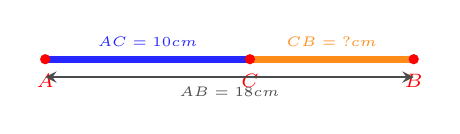
\begin{tikzpicture}[scale=0.65]
  \draw[line width=2.5pt, blue!85] (0,0) -- (4,0) node[midway, above, font=\bfseries\tiny] {$AC = 10\text{ cm}$};
  \draw[line width=2.5pt, orange!90] (4,0) -- (7.2,0) node[midway, above, font=\bfseries\tiny] {$CB = \text{? cm}$};
  \fill[red] (0,0) circle (0.1cm) node[below=2pt, font=\bfseries\scriptsize] {$A$};
  \fill[red] (4,0) circle (0.1cm) node[below=2pt, font=\bfseries\scriptsize] {$C$};
  \fill[red] (7.2,0) circle (0.1cm) node[below=2pt, font=\bfseries\scriptsize] {$B$};
  \draw[line width=0.8pt, stealth-stealth, black!70] (0,-0.35) -- (7.2,-0.35) node[midway, below, font=\bfseries\tiny] {$AB = 18\text{ cm}$};
\end{tikzpicture}
\end{center}
Đoạn thẳng $CB$ dài là:
\begin{multicols}{4}
\choice
{\True $8\text{ cm}$}
{$7\text{ cm}$}
{$9\text{ cm}$}
{$10\text{ cm}$}
\end{multicols}
\loigiai{
Độ dài đoạn $CB$ là: $18 - 10 = 8\text{ cm}$.\\
\textbf{Đáp án: A.}
}
\end{ex}

\newpage
% --- TRANG 4: CÂU 13 ĐẾN CÂU 16 (ĐÚNG / SAI) ---

\textbf{Phần 2. Trắc nghiệm đúng sai}
\setcounterpageref{ex}{0}

% CÂU 13: Các phép tính độ dài
\begin{ex} %[1H7H28]
Các phép toán đo độ dài trong phiếu bài tập:
\begin{center}
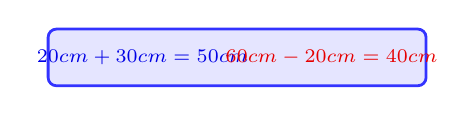
\begin{tikzpicture}[scale=0.6]
  \draw[fill=blue!10, draw=blue!80, line width=1pt, rounded corners=3pt] (-4,-0.6) rectangle (4,0.6);
  \node[font=\bfseries\scriptsize, color=blue!90!black] at (-2,0) {$20\text{ cm} + 30\text{ cm} = 50\text{ cm}$};
  \node[font=\bfseries\scriptsize, color=red!90!black] at (2,0) {$60\text{ cm} - 20\text{ cm} = 40\text{ cm}$};
\end{tikzpicture}
\end{center}
Xét tính đúng hoặc sai của các khẳng định sau:
\choiceTF
{\True Phép tính $20\text{ cm} + 30\text{ cm} = 50\text{ cm}$ là đúng.}
{\True Phép tính $60\text{ cm} - 20\text{ cm} = 40\text{ cm}$ là đúng.}
{Phép tính $45\text{ cm} + 5\text{ cm} = 60\text{ cm}$ là đúng.}
{\True Phép tính $45\text{ cm} + 5\text{ cm} = 50\text{ cm}$ là đúng.}
\loigiai{
\begin{itemize}
  \item a) \textbf{Đúng}: $20 + 30 = 50\text{ cm}$.
  \item b) \textbf{Đúng}: $60 - 20 = 40\text{ cm}$.
  \item c) \textbf{Sai}: $45 + 5 = 50\text{ cm}$ (chứ không phải $60\text{ cm}$).
  \item d) \textbf{Đúng}: $45 + 5 = 50\text{ cm}$.
\end{itemize}
}
\end{ex}

% CÂU 14: Hai đoạn thẳng 25 cm và 15 cm
\begin{ex} %[1H7V28]
Cho hai đoạn thẳng: đoạn thứ nhất dài $25\text{ cm}$, đoạn thứ hai dài $15\text{ cm}$:
\begin{center}
\begin{tikzpicture}[scale=0.6]
  \draw[fill=cyan!30, draw=black] (0,0.3) rectangle (5.0,0.7) node[midway, font=\tiny\bfseries] {Đoạn $1$: $25\text{ cm}$};
  \draw[fill=orange!30, draw=black] (0,-0.3) rectangle (3.0,0.1) node[midway, font=\tiny\bfseries] {Đoạn $2$: $15\text{ cm}$};
\end{tikzpicture}
\end{center}
Xét tính đúng hoặc sai của các nhận xét sau:
\choiceTF
{\True Tổng độ dài của hai đoạn thẳng là $40\text{ cm}$.}
{\True Đoạn thứ nhất dài hơn đoạn thứ hai là $10\text{ cm}$.}
{Tổng độ dài hai đoạn thẳng ngắn hơn $35\text{ cm}$.}
{\True Tổng độ dài hai đoạn thẳng dài hơn $35\text{ cm}$.}
\loigiai{
\begin{itemize}
  \item a) \textbf{Đúng}: $25 + 15 = 40\text{ cm}$.
  \item b) \textbf{Đúng}: $25 - 15 = 10\text{ cm}$.
  \item c) \textbf{Sai}: $40\text{ cm} > 35\text{ cm}$ (không thể ngắn hơn).
  \item d) \textbf{Đúng}: $40\text{ cm} > 35\text{ cm}$.
\end{itemize}
}
\end{ex}

% CÂU 15: Quy tắc đo trên thước kẻ
\begin{ex} %[1H7H28]
Hình minh họa thước kẻ xăng-ti-mét:
\begin{center}
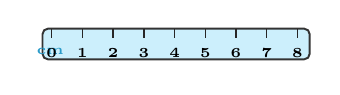
\begin{tikzpicture}[scale=0.6]
  \VeThuocCmMini[cyan]{8}{0,0}
\end{tikzpicture}
\end{center}
Xét tính đúng hoặc sai của các phát biểu về thước kẻ:
\choiceTF
{\True Khoảng cách từ vạch $0$ đến vạch $1$ là $1\text{ cm}$.}
{\True Khoảng cách từ vạch $0$ đến vạch $5$ là $5\text{ cm}$.}
{Khoảng cách từ vạch $2$ đến vạch $6$ là $6\text{ cm}$.}
{\True Khoảng cách từ vạch $2$ đến vạch $6$ là $4\text{ cm}$.}
\loigiai{
\begin{itemize}
  \item a) \textbf{Đúng}: Từ $0$ đến $1$ là $1\text{ cm}$.
  \item b) \textbf{Đúng}: Từ $0$ đến $5$ là $5\text{ cm}$.
  \item c) \textbf{Sai}: Từ $2$ đến $6$ là $6 - 2 = 4\text{ cm}$.
  \item d) \textbf{Đúng}: $6 - 2 = 4\text{ cm}$.
\end{itemize}
}
\end{ex}

% CÂU 16: So sánh các số đo
\begin{ex} %[1H7V28]
Bốn thẻ so sánh độ dài:
\begin{center}
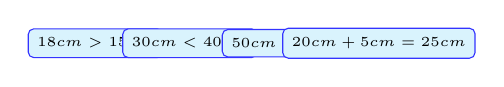
\begin{tikzpicture}[scale=0.6]
  \node[draw=blue!80, fill=cyan!15, rounded corners=2pt, font=\bfseries\tiny] at (-3,0) {$18\text{ cm} > 15\text{ cm}$};
  \node[draw=blue!80, fill=cyan!15, rounded corners=2pt, font=\bfseries\tiny] at (-1,0) {$30\text{ cm} < 40\text{ cm}$};
  \node[draw=blue!80, fill=cyan!15, rounded corners=2pt, font=\bfseries\tiny] at (1,0) {$50\text{ cm} = 5\text{ cm}$};
  \node[draw=blue!80, fill=cyan!15, rounded corners=2pt, font=\bfseries\tiny] at (3,0) {$20\text{ cm} + 5\text{ cm} = 25\text{ cm}$};
\end{tikzpicture}
\end{center}
Xét tính đúng hoặc sai của các so sánh sau:
\choiceTF
{\True $18\text{ cm} > 15\text{ cm}$ là đúng.}
{\True $30\text{ cm} < 40\text{ cm}$ là đúng.}
{Phép so sánh $50\text{ cm} = 5\text{ cm}$ là đúng.}
{\True $20\text{ cm} + 5\text{ cm} = 25\text{ cm}$ là đúng.}
\loigiai{
\begin{itemize}
  \item a) \textbf{Đúng}: $18 > 15$.
  \item b) \textbf{Đúng}: $30 < 40$.
  \item c) \textbf{Sai}: $50\text{ cm} > 5\text{ cm}$.
  \item d) \textbf{Đúng}: $20 + 5 = 25\text{ cm}$.
\end{itemize}
}
\end{ex}

\newpage
% --- TRANG 5: CÂU 17 ĐẾN CÂU 20 (TRẢ LỜI NGẮN / ĐIỀN SỐ) ---

\textbf{Phần 3. Trả lời ngắn}
\setcounterpageref{ex}{0}

% CÂU 17: Tính 12 cm + 7 cm
\begin{ex} %[1H7H28]
Thực hiện phép tính độ dài:
\begin{center}

\begin{tikzpicture}[scale=0.65]
  \draw[fill=yellow!30, draw=blue!80, line width=0.7pt, rounded corners=2pt] (-2.2,-0.4) rectangle (2.2,0.4);
  \node[font=\bfseries\normalsize, color=blue!90!black] at (0,0) {$12\text{ cm} + 7\text{ cm} = \dots\text{ cm}$};
\end{tikzpicture}
\end{center}
Kết quả của phép tính là bao nhiêu xăng-ti-mét?
\textit{Trả lời:} \raisebox{-2pt}{\tcbox[colframe=blue!80!black,colback=white,size=small,arc=3pt]{$19$}}
\loigiai{
$12 + 7 = 19\text{ cm}$.\\
\textbf{Đáp số: $19$.}
}
\end{ex}

% CÂU 18: Tính 18 cm - 8 cm
\begin{ex} %[1H7H28]
Thực hiện phép tính độ dài:
\begin{center}

\begin{tikzpicture}[scale=0.65]
  \draw[fill=pink!30, draw=red!80, line width=0.7pt, rounded corners=2pt] (-2.2,-0.4) rectangle (2.2,0.4);
  \node[font=\bfseries\normalsize, color=red!90!black] at (0,0) {$18\text{ cm} - 8\text{ cm} = \dots\text{ cm}$};
\end{tikzpicture}
\end{center}
Kết quả của phép tính là bao nhiêu xăng-ti-mét?
\textit{Trả lời:} \raisebox{-2pt}{\tcbox[colframe=blue!80!black,colback=white,size=small,arc=3pt]{$10$}}
\loigiai{
$18 - 8 = 10\text{ cm}$.\\
\textbf{Đáp số: $10$.}
}
\end{ex}

% CÂU 19: Cắt bớt đoạn dây
\begin{ex} %[1H7V28]
Đoạn dây dài $35\text{ cm}$, cắt bớt đi $15\text{ cm}$:
\begin{center}
\begin{tikzpicture}[scale=0.65]
  \draw[line width=2pt, green!70!black] (0,0) -- (3.2,0) node[midway, above, font=\bfseries\tiny] {Còn lại ? cm};
  \draw[line width=2pt, gray!60, dashed] (3.2,0) -- (5.6,0) node[midway, above, font=\bfseries\tiny] {Cắt $15\text{ cm}$};
  \draw[line width=0.8pt, stealth-stealth, blue!85] (0,-0.35) -- (5.6,-0.35) node[midway, below, font=\bfseries\tiny] {Cả đoạn dây $35\text{ cm}$};
\end{tikzpicture}
\end{center}
Hỏi đoạn dây còn lại dài bao nhiêu xăng-ti-mét?
\textit{Trả lời:} \raisebox{-2pt}{\tcbox[colframe=blue!80!black,colback=white,size=small,arc=3pt]{$20$}}
\loigiai{
Đoạn dây còn lại dài là: $35 - 15 = 20\text{ cm}$.\\
\textbf{Đáp số: $20$.}
}
\end{ex}

% CÂU 20: Vận dụng cao - Tính nhanh nhóm số đo
\begin{ex} %[1H7C28]
Tính nhanh tổng độ dài các thanh gỗ:
\begin{center}

\begin{tikzpicture}[scale=0.65]
  \draw[fill=yellow!70!orange, draw=black, line width=0.8pt, rounded corners=3pt] (-3.8,-0.45) rectangle (3.8,0.45);
  \node[font=\bfseries\small, color=blue!95!black] at (0,0) {
    $20\text{ cm} + 15\text{ cm} + 30\text{ cm} + 5\text{ cm} = \text{\textbf{?}}\text{ cm}$
  };
\end{tikzpicture}
\end{center}
Kết quả của phép tính nhanh trên là bao nhiêu xăng-ti-mét?
\textit{Trả lời:} \raisebox{-2pt}{\tcbox[colframe=blue!80!black,colback=white,size=small,arc=3pt]{$70$}}
\loigiai{
Nhóm các số tròn chục và số có tổng tròn chục:\\
$(20 + 30) + (15 + 5) = 50 + 20 = 70\text{ cm}$.\\
\textbf{Đáp số: $70$.}
}
\end{ex}
